\newpage
\def\thoigian{90}%--Thời gian
\de{Đề số 3}{Chương V. Phương trình mặt phẳng, đường thẳng, mặt cầu}

\begin{center}
	\textbf{PHẦN 1 - Câu trắc nghiệm nhiều phương án lựa chọn.}
\end{center}
\setcounter{ex}{0}
\Opensolutionfile{ans}[ans-ABCD]
%Câu 1
\begin{ex}%[2H5N1-1]%[Dự án D - đợt 2 NH 24-25 - Xuan Vy Pham]
	Trong không gian $Oxyz$, điểm nào dưới đây \textbf{không thuộc} $(\alpha)\colon x+y+z-6=0$?
	\choice
	{$N(2;2;2)$}
	{\True $M(3;-1;-2)$}
	{$P(1;2;3)$}
	{$M(1;-1;1)$}
	\loigiai{
		Ta có $3-1-2-6\ne 0$ nên $M\notin (\alpha)$.
	}
\end{ex}
%Câu 2
\begin{ex}%[2H5N1-2]%[Dự án D - đợt 2 NH 24-25 - Xuan Vy Pham]
	Trong không gian $Oxyz$, một vectơ pháp tuyến của mặt phẳng $(Oxy)$ có tọa độ là
	\choice
	{$(1;1;0)$}
	{\True $(0;0;1)$}
	{$(0;1;0)$}
	{$(1;1;1)$}
	\loigiai{
	Một vectơ pháp tuyến của mặt phẳng $(Oxy)$ có tọa độ là $(0;0;1)$.
	}
\end{ex}
%Câu 3
\begin{ex}%[2H5N1-2]%[Dự án D - đợt 2 NH 24-25 - Xuan Vy Pham]
	Trong không gian $Oxyz$, cho ba điểm $A(2;-1;3)$, $B(4;0;1)$ và $C(-10;5;3)$. Vectơ nào dưới đây là một vectơ pháp tuyến của mặt phẳng $(ABC)$?
	\choice
	{$\overrightarrow{n}_1=(1;8;2)$}
	{$\overrightarrow{n}_2=(1;2;0)$}
	{$\overrightarrow{n}_3=(1;2;2)$}
	{\True $\overrightarrow{n}_4=(1;-2;2)$}
	\loigiai{
		Ta có $\overrightarrow{AB}=(2;1;-2)$ và $\overrightarrow{AC}=(-12;6;0)$ nên $\left[\overrightarrow{AB},\overrightarrow{AC}\right]=(12;-24;24)=12(1;-2;2)$.\\
		Do đó $\overrightarrow{n}_4=(1;-2;2)$ là một vectơ pháp tuyến của mặt phẳng $(ABC)$.
	}
\end{ex}
%Câu 4
\begin{ex}%[2H5H1-3]%[Dự án D - đợt 2 NH 24-25 - Xuan Vy Pham]
	Trong không gian $Ox y z$, cho hai điểm $A(0; 1; 1)$ và $B(1; 2; 3)$. Phương trình của mặt phẳng $(P)$ đi qua $A$ và vuông góc với đường thẳng $AB$ là
	\choice
	{\True $x+y+2z-3=0$}
	{$x+y+2z-6=0$}
	{$x+3y+4z-7=0$}
	{$x+3y+4z-26=0$}
	\loigiai{
		Ta có $AB\perp (P)\Rightarrow \overrightarrow{AB}=(1;1;2)$ là vectơ pháp tuyến của mặt phẳng $(P)$.\\
		Khi đó, mặt phẳng $(P)$ qua $A(0;1;1)$ nên có phương trình \begin{align*}
			x+y+2z-3=0.
		\end{align*}
	}
\end{ex}
%Câu 5
\begin{ex}%[2H5N2-2]%[Dự án D - đợt 2 NH 24-25 - Xuan Vy Pham]
	Trong không gian $Oxyz$, cho hai điểm $A(1;1;0)$ và $B(0;1;2)$. Vectơ nào dưới đây là một vectơ chỉ phương của đường thẳng $AB$?
	\choice
	{\True $\overrightarrow{b}=(-1;0;2)$}
	{$\overrightarrow{c}=(1;2;2)$}
	{$\overrightarrow{d}=(-1;1;2)$}
	{$\overrightarrow{a}=(-1;0;-2)$}
	\loigiai{
		Ta có $\overrightarrow{AB}=(-1;0;2)=\overrightarrow{b}$ là một vectơ chỉ phương của đường thẳng $AB$.
	}
\end{ex}
%Câu 6
\begin{ex}%[2H5N2-1]%[Dự án D - đợt 2 NH 24-25 - Xuan Vy Pham]
	Trong không gian $Oxyz$, điểm nào dưới đây thuộc đường thẳng $d\colon \heva{&x=1-t\\&y=2+3t\\&z=1+3t}$?
	\choice
	{$P(-1;2;1)$}
	{$Q(1;-2;-1)$}
	{\True $N(0;5;4)$}
	{$M(1;2;-1)$}
	\loigiai{
		Ta có $\heva{&0=1-t\\&5=2+3t\\&4=1+3t}\Leftrightarrow t=1$ nên $N \in d$.
	}
\end{ex}
%Câu 7
\begin{ex}%[2H5N2-7]%[Dự án D - đợt 2 NH 24-25 - Xuan Vy Pham]
	Góc giữa đường thẳng $d\colon \dfrac{x}{1}=\dfrac{y}{2}=\dfrac{z-1}{-1}$ và mặt phẳng $(P)\colon x-y+2z-1=0$ bằng
	\choice
	{\True $30^\circ$}
	{$120^\circ$}
	{$45^\circ$}
	{$60^\circ$}
	\loigiai{Đường thẳng $d$ có vectơ chỉ phương là $\overrightarrow{u}=(1;2;-1)$, mặt phẳng $(P)$ có vectơ pháp tuyến là $\overrightarrow{n}=(1;-1;2)$.\\
		Ta có $$\sin (d,(P))=\dfrac{\left|\overrightarrow{u}\cdot\overrightarrow{n}\right|}{\left|\overrightarrow{u}\right|\cdot\left|\overrightarrow{n}\right|}=\dfrac{|1\cdot 1+2\cdot(-1)+(-1)\cdot2|}{\sqrt{1^2+2^2+(-1)^2}\cdot\sqrt{1^2+(-1)^2+2^2}}=\dfrac{1}{2}.$$
		Suy ra $(d,(P))=30^\circ$.}
\end{ex}
%Câu 8
\begin{ex}%[2H5H2-3]%[Dự án D - đợt 2 NH 24-25 - Xuan Vy Pham]
	Trong không gian $Oxyz$, phương trình đường trung tuyến $AM$ của tam giác $ABC$ với $A(3;1;2), B(-3; 2; 5), C(1; 6;-3)$ là
	\choice
	{$\heva{&x=1+t \\& y=-1-3t \\& z=8-4t}$}
	{$\heva{&x=1-4t \\& y=-3+3t \\& z=4-1t}$}
	{\True $\heva{&x=3-4t \\& y=1+3t \\& z=2-t}$}
	{$\heva{&x=1+3t \\& y=-3+4t \\& z=4-t}$}
	\loigiai{
		$M$ là trung điểm $BC$ nên $M(-1;4;1)$.\\
		Đường trung tuyến $AM$ đi qua điểm $A$ và nhận $\overrightarrow{AM}=(-4;3;-1)$ làm vectơ chỉ phương nên có phương trình tham số là $\heva{&x=3-4t \\& y=1+3t \\& z=2-t}$,  $t\in\mathbb{R}$.
	}
\end{ex}
%Câu 9
\begin{ex}%[2H5N3-2]%[Dự án D - đợt 2 NH 24-25 - Xuan Vy Pham]
	Trong không gian $Oxyz$, mặt cầu $(S) \colon (x-1)^2+(y-2)^2+(z+3)^2=9$ có tọa độ tâm là
	\choice
	{$(-1;-2;3)$}
	{$(-2;-4;6)$}
	{\True $(1;2;-3)$}
	{$(2;4;-6)$}
	\loigiai{
		Mặt cầu $(S)$ có tâm $I(1;2;-3)$.
	}
\end{ex}
%Câu 10
\begin{ex}%[2H5N3-2]%[Dự án D - đợt 2 NH 24-25 - Xuan Vy Pham]
	Trong không gian $Oxyz$, mặt cầu $(S): x^2+y^2+z^2-4x+2z+4=0$ có tâm và bán kính là 
	\choice
	{$I(2;0;-1)$; $R=3$}
	{$I(4;0;-2)$; $R=3$}
	{$I(-2;0;1)$; $R=1$}
	{\True $I(2;0;-1)$; $R=1$}
	\loigiai{
		Mặt cầu $(S)$ có tâm $I(2;0;-1)$ bán kính $R=\sqrt{2^2+0^2+(-1)^2-4}=1$.
	}
\end{ex}
%Câu 11
\begin{ex}%[2H5H3-3]%[Dự án D - đợt 2 NH 24-25 - Xuan Vy Pham]
	Trong không gian $Oxyz$, mặt cầu $(S)$ có tâm $I(1;2;-4)$, thể tích bằng $36\pi$. Phương trình của mặt cầu $(S)$ là
	\choice
	{\True $(x-1)^2+(y-2)^2+(z+4)^2=9$}
	{$(x-1)^2+(y-2)^2+(z-4)^2=9$}
	{$(x+1)^2+(y+2)^2+(z-4)^2=9$}
	{$(x-1)^2+(y-2)^2+(z+4)^2=3$}
	\loigiai{
		Mặt cầu có thể tích là $36\pi$ nên $\dfrac{4}{3}\pi R^3=36\pi \Leftrightarrow R=3$.\\
		Phương trình mặt cầu tâm $I$, bán kính $R$ là $(x-1)^2+(y-2)^2+(z+4)^2=9$.
	}
\end{ex}
%Câu 12
\begin{ex}%[2H5H3-3]%[Dự án D - đợt 2 NH 24-25 - Xuan Vy Pham]
	Trong không gian $Oxyz$, cho điểm $I(1;-2;3)$. Hỏi phương trình nào sau đây là phương trình mặt cầu $(S)$ có tâm $I$ và tiếp xúc với trục tung $Oy$?
	\choice
	{$(x-1)^2+(y+2)^2+(z-3)^2=\sqrt{10}$}
	{\True $(x-1)^2+(y+2)^2+(z-3)^2=10$}
	{$(x+1)^2+(y-2)^2+(z+3)^2=10$}
	{$(x-1)^2+(y+2)^2+(z-3)^2=9$}
	\loigiai{
		Gọi $H$ là hình chiếu của $I$ lên $Oy$, ta có $H(0;-2;0)$.\\
		Ta có $\overrightarrow{IH}=(-1;0;-3) \Rightarrow R=IH=\sqrt{10}$.\\
		Phương trình mặt cầu $(S): (x-1)^2+(y+2)^2+(z-3)^2=10$.
	}
\end{ex}
\Closesolutionfile{ans}
%\indapan{6}{ans-ABCD}
%\cauds
\begin{center}
	\textbf{PHẦN 2 - Câu trắc nghiệm đúng sai. Trong mỗi ý a, b, c, d ở mỗi câu, thí sinh chọn đúng hoặc sai}
\end{center}
\setcounter{ex}{0}
\Opensolutionfile{ans}[ans-DS]
%Câu 1
\begin{ex}%[2H5V2-3]%[Dự án D - đợt 2 NH 24-25 - Xuan Vy Pham]
	Trong không gian $Oxyz$, cho phương trình của đường thẳng $d\colon \dfrac{x-1}{1}=\dfrac{y}{-2}=\dfrac{z+3}{2}$ và mặt phẳng $(P)\colon 3x+y+z=0$.
	\choiceTF
	{Điểm $A(1; 0; 3)$ thuộc đường thẳng $d$}
	{\True Đường thẳng $d$ không vuông góc với mặt phẳng $(P)$}
	{Giao điểm của đường thẳng $d$ và $(P)$ là điểm $M(a; b; c)$. Khi đó $a+b+c=-1$}
	{\True Gọi $d'$ là đường thẳng nằm trong mặt phẳng $(P)$, đồng thời $d'$ cắt và vuông góc với $d$. Khi đó đường thẳng $d'$ có một vectơ chỉ phương là $\overrightarrow{u}=(4;-5;-7)$}
	\loigiai{
		\begin{itemchoice}
			\itemch  \textbf{Sai}.\\
			Điểm $A(1; 0; 3)$ không thuộc đường thẳng $d$ vì $\dfrac{1-1}{1}=\dfrac{0}{-2}\ne \dfrac{3+3}{2}$.
			\itemch  \textbf{Đúng}.\\
			Đường thẳng $d\colon \dfrac{x-1}{1}=\dfrac{y}{-2}=\dfrac{z+3}{2}$ có vectơ chỉ phương $\overrightarrow{u}=(1;-2;2)$.\\
			Mặt phẳng $(P)\colon 3x+y+z=0$ có vectơ pháp tuyến $\overrightarrow{n}=(3;1;1)$.\\
			Ta thấy $\dfrac{1}{3}\ne \dfrac{-2}{1}\ne \dfrac{2}{1}$ nên $d$ không vuông góc với mặt phẳng $(P)$.
			\itemch  \textbf{Sai}.\\
			Tọa độ $M$ là nghiệm của hệ phương trình $\heva{&x=1+t\\&y=-2t\\&z=-3+2t\\&3x+y+z=0}\Leftrightarrow \heva{&x=1\\&y=0\\&z=-3\\&t=0.}$\\
			Suy ra $M(1;0;-3)$. Vậy $a+b+c=-2$
			\itemch  \textbf{Đúng}.\\
			Vì $d'$ là đường thẳng nằm trong mặt phẳng $(P)$, đồng thời $d'$ cắt và vuông góc với $d$ nên $d'$ qua $M(1;0;-3)$ và có vectơ chỉ phương $\overrightarrow{u}=\left[\overrightarrow{u}_d,\overrightarrow{n}_{P}\right]=-(4;-5;-7)$.
		\end{itemchoice}
	}
\end{ex}
%Câu 2
\begin{ex}%[2H5H3-2]%[Dự án D - đợt 2 NH 24-25 - Xuan Vy Pham]
	Trong không gian $Oxyz$, cho hai điểm $A(0;1;1)$, $B(1;0;-3)$, $C(-1;-2;-3)$ và mặt cầu $(S)$ có phương trình là $x^2+y^2+z^2-2x+2z-2=0$. 
	\choiceTF
	{\True Mặt cầu $(S)$ có bán kính là $2$}
	{Mặt phẳng $(ABC)$ có phương trình $2x-2y+z-1=0$}
	{Khoảng cách từ tâm mặt cầu $(S)$ đến mặt phẳng $(ABC)$ bằng $\dfrac{1}{3}$}
	{\True Mặt phẳng $(ABC)$ cắt mặt cầu $(S)$ theo một đường tròn có bán kính bằng $\dfrac{4\sqrt{2}}{3}$}
	\loigiai{
		\begin{itemchoice}
			\itemch  \textbf{Đúng}.
			Bán kính mặt cầu $(S)$ là $R=\sqrt{1^2+(-1)^2-\left(-2\right)}=2$.			 
			\itemch  \textbf{Sai}.
			Ta có $\overrightarrow{AB}=(1;-1;-4)$, $\overrightarrow{AC}=(-1;-3;-4)$.\\
			$\Rightarrow\left[\overrightarrow{AB};\overrightarrow{AC}\right]=(-8;8;-4)=-4(2;-2;1)$.\\
			Suy ra $\overrightarrow{n}_{(ABC)}= (2;-2;1)$.\\
			Phương trình mặt phẳng $(ABC)$ là $2x-2(y-1)+(z-1)=0 \Leftrightarrow 2x-2y+z+1=0$.
			\itemch  \textbf{Sai}. Tọa độ tâm $I$ của mặt cầu $(S)$ là $I(1;0;-1)$.\\
			Ta có $\mathrm{d}(I,(ABC))=\dfrac{\left|2\cdot 1-2\cdot 0-1+1\right|}{\sqrt{2^2+(-2)^2+1}}=\dfrac{2}{3}$.
			\itemch \textbf{Đúng}.
			Bán kính đường tròn cắt $(S)$ theo mặt phẳng $(ABC)$ là $$r=\sqrt{R^2-\mathrm{d^{2}}(I,(ABC))}=\dfrac{4\sqrt{2}}{3}.$$	
		\end{itemchoice}
	}
\end{ex}
\Closesolutionfile{ans}
\begin{center}
	\textbf{PHẦN 3 - Câu trắc nghiệm trả lời ngắn}
\end{center}
\setcounter{ex}{0}
%Câu 1
\begin{ex}%[2H5H2-7]%[Dự án D - đợt 2 NH 24-25 - Xuan Vy Pham]
	Trên một sân khấu đã thiết lập sẵn một hệ toạ độ $Oxyz$, tính góc giữa tia sáng có phương trình $d\colon \heva{& x=2\\& y=1+t\\& z=1+t}$ và mặt sàn sân khấu có phương trình $z=0$.
	\shortans{$45$}
	\loigiai{
		$d$ có vectơ chỉ phương $\overrightarrow{u}=(0;1;1)$.\\
		Mặt sàn sân khấu là mặt phẳng có vectơ pháp tuyến $\overrightarrow{k}=(0;0;1)$.\\
		Gọi góc giữa tia sáng và mặt sàn sân khấu là $\alpha$.\\
		Khi đó $\sin\alpha = \dfrac{\left|\overrightarrow{u}\cdot\overrightarrow{k}\right|}{\left|\overrightarrow{u}\right|\cdot\left|\overrightarrow{k}\right|} = \dfrac{\left|0\cdot 0+1\cdot 0+1\cdot 1\right|}{\sqrt{2}\cdot 1}= \dfrac{1}{\sqrt{2}}$.\\
		Suy ra $\alpha=45^\circ$.
	}
\end{ex}
%Câu 2
\begin{ex}%[2H5V1-7]%[Dự án D - đợt 2 NH 24-25 - Xuan Vy Pham]
Một sân vận động được xây dựng theo mô hình là hình chóp cụt $OAGD.BCFE$ có hai đáy song song với nhau. Mặt sân $OAGD$ là hình chữ nhật và được gắn hệ trục $Oxyz$ như hình vẽ (đơn vị trên mỗi trục tọa độ là mét). Mặt sân $OAGD$ có chiều dài $OA=100$\,m, chiều rộng $OD=60$\,m và tọa độ điểm $B(10;10;1)$. Giả sử phương trình tổng quát của mặt phẳng $(OACB)$ có dạng $ax+y+cz+d=0$. Giá trị biểu thức $a+c+d$ bằng bao nhiêu?	
\begin{center}
	\begin{tikzpicture}[scale=0.9, font=\footnotesize, line join=round, line cap=round,>=stealth]
		\path 
		(0,0) coordinate (O)
		(30:5) coordinate (A)
		(80:2.5) coordinate (B)
		(50:5) coordinate (C)
		(150:4) coordinate (D)
		(120:4) coordinate (E)
		(75:3.5) coordinate (G)
		++(80:1) coordinate (F)
		;
		\fill[cyan!30,opacity=.5] 
		(O)--(B)--(C)--(A)--cycle
		(O)--(B)--(E)--(D)--cycle
		(B)--(E)--(F)--(C)--cycle;
		\draw[->,red,thick] (O)--($(O)+(30:6)$) node[below]{$x$};
		\draw[->,red,thick] (O)--($(O)+(90:5)$) node[left]{$z$};
		\draw[->,red,thick] (O)--($(O)+(150:5)$) node[below]{$y$};
		\draw 
		(C)--(B)--(E)--(F)--cycle
		(D)--(E) (O)--(B) (C)--(A);
		\draw[dashed] (D)--(G)--(A) (F)--(G);
		\foreach \x/\g in {O/-90,A/-90,B/90,C/90,D/-90,E/90,F/90,G/30}{\fill (\x) circle (1pt)+(\g:3mm)node{$\x$};};
	\end{tikzpicture}
\end{center}
\par
\shortans{$-10$}
\loigiai{
	Theo hình vẽ ta có $A\in Ox$ và $OA=100$\,m nên ta có $A(100,0,0)$.\\
	Ta có $\overrightarrow{OA}=(100,0,0)$ và $\overrightarrow{OB}=(10;10;1)$.\\
	Khi đó $\left[\overrightarrow{OA},\overrightarrow{OB}\right]=(0,-100,1000)$.\\
	Mặt phẳng $(OACB)$ đi qua $A(100,0,0)$ và có một vectơ pháp tuyến là $\overrightarrow{n}=(0,1,-10)$.\\
	Phương trình tổng quát của $(OACB)$ là 
	\[0\cdot (x-100)+1\cdot (y-0)-10\cdot (z-0)=0\Leftrightarrow y-10z=0.\]
	Suy ra $a=0$, $c=-10$, $d=0$.\\
	Vậy $a+c+d=-10$.
}
\end{ex}
%Câu 3...........................
\begin{ex}%[2H5H3-4]%[Dự án D - đợt 2 NH 24-25 - Xuan Vy Pham]
	\immini{
		Người ta muốn thiết kế một bồn chứa khí hoá lỏng hình cầu bằng phần mềm 3D. Cho biết phương trình bề mặt của bồn chứa là 
		$(S) \colon  (x-6)^2+(y-6)^2+(z-6)^2=25$. Phương trình mặt phẳng chứa nắp là $(P) \colon  z=10$. Tính khoảng cách từ tâm bồn chứa đến mặt phẳng chứa nắp.
	}
	{
		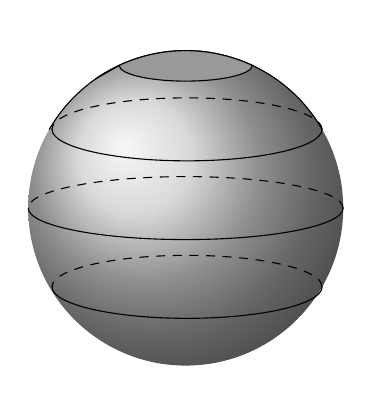
\begin{tikzpicture}[scale=1,>=stealth, font=\footnotesize, line join=round, line cap=round]
			\path
			(0,0) coordinate (O)
			(30:2) coordinate (A)
			(-30:2) coordinate (B)
			(65:2) coordinate (C)
			(125:2) coordinate (C')
			;
			\pgfresetboundingbox
			\shade [ball color=gray!40] (O) circle (2);
			\draw (A) arc (30:150:2) ;
			\draw[dashed] (A) arc (0:180: 1.715 and 0.4);
			\draw (A) arc (0:-180: 1.715 and 0.4);
			\draw[dashed] (B) arc (0:180: 1.715 and 0.4);
			\draw (B) arc (0:-180: 1.715 and 0.4);
			\draw[dashed] (2,0) arc (0:180: 2 and 0.4);
			\draw (2,0) arc (0:-180: 2 and 0.4);
			\draw[fill=gray!80] (C) arc (0:-180: {2*cos(65)} and 0.2) --  (C')  arc (125:65:2);
			%\foreach \x/\g in {A/180,B/90,A'/0,O/-90}
			%\fill[black] (\x) circle(1.1pt) + (\g:3mm) node {$\x$};
		\end{tikzpicture}
	}
	\shortans{$4$}
	\loigiai{
		$(S)$ có tâm $I(6;6;6)$ và bán kính $R=5$.  \\
		Khoảng cách từ tâm bồn chứa đến mặt phẳng chứa nắp là
		\[
		\mathrm{d}(I, (P)) = \dfrac{|6-10|}{1} = 4.
		\]
	}
\end{ex}
%Câu 4
\begin{ex}%[2H5V3-4]%[Dự án D - đợt 2 NH 24-25 - Xuan Vy Pham]
\immini{
	Bạn Bình đố bạn Nam tìm được đường kính của quả bóng rổ, biết rằng nếu đặt quả bóng ở một góc căn phòng hình hộp chữ nhật, sao cho quả bóng chạm (tiếp xúc) với hai bức tường và nền nhà của căn phòng đó (khi đó khoảng cách từ tâm quả bóng đến hai bức tường và nền nhà đều bằng bán kính của quả bóng) thì có một điểm $M$ trên quả bóng với khoảng cách lần lượt đến hai bức tường và nền nhà là $17$ cm, $18$ cm và $21$ cm (tham khảo hình vẽ bên). Hãy giúp Nam xác định đường kính của quả bóng rổ đó. Biết rằng loại bóng rổ tiêu chuẩn có đường kính từ $23$ cm đến $24{,}5$ cm (làm tròn đến một chữ số thập phân sau dấu phẩy).
}
{
	\begin{tikzpicture}[scale=1,>=stealth, font=\footnotesize, line join=round, line cap=round]
		\path
		(0,0) coordinate (O)
		(2.77,1.75) coordinate (A)
		(-0.55,1.87) coordinate (B)
		(1,-1.67) coordinate (C) 
		(4,-1) coordinate (x) 
		(-4,-0.55) coordinate (y) 
		(0,4) coordinate (z) 
		(0.28,0.51) coordinate (I) 
		(1,1.4) coordinate (M) 
		;
		\pgfresetboundingbox
		\shade [ball color=brown] (I) circle (2);
		\draw (M)--(A) (M)--(B) (M)--(C) (O)--(x) (O)--($(O)!0.66!(y)$) (O)--(z);
		\foreach \x/\g in {A/40,B/140,C/-90,M/90}
		\fill[black] (\x) circle(1.1pt) + (\g:3mm) node {$\x$};
	\end{tikzpicture}
}
\shortans{$23{,}9$}
\loigiai{
	\begin{center}
		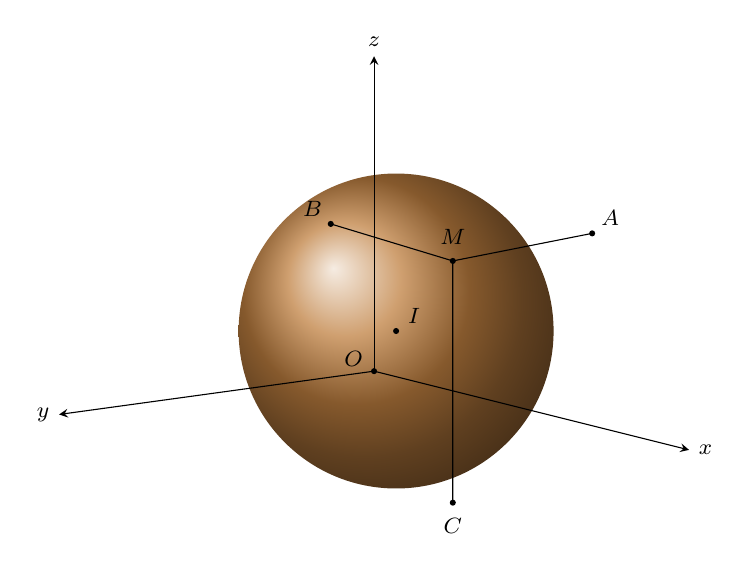
\begin{tikzpicture}[scale=1,>=stealth, font=\footnotesize, line join=round, line cap=round]
			\path
			(0,0) coordinate (O)
			(2.77,1.75) coordinate (A)
			(-0.55,1.87) coordinate (B)
			(1,-1.67) coordinate (C) 
			(4,-1) coordinate (x) 
			(-4,-0.55) coordinate (y) 
			(0,4) coordinate (z) 
			(0.28,0.51) coordinate (I) 
			(1,1.4) coordinate (M) 
			;
			\shade [ball color=brown] (I) circle (2);
			\draw[->] (O)--(x) node[right]{$x$} ;
			\draw[->] (O)--(y) node[left]{$y$} ;
			\draw[->] (O)--(z) node[above]{$z$} ;
			\draw (M)--(A) (M)--(B) (M)--(C) ;
			\foreach \x/\g in {A/40,B/140,C/-90,M/90,O/150,I/40}
			\fill[black] (\x) circle(1.1pt) + (\g:3mm) node {$\x$};
		\end{tikzpicture}
	\end{center}
	Chọn hệ trục tọa độ $Oxyz$ như hình vẽ. \\
	Gọi $I(a;b;c)$ là tâm của quả bóng. \\
	Ta có $M(18;17;21)$. \\
	Vì quả bóng tiếp xúc với các bức tường và nền nhà nên $a=b=c$ ($a>0$, $b>0$, $c>0$). \\
	Mặt cầu đi qua $M$ nên $a=IM= \sqrt{(a-18)^2+(b-17)^2+(c-21)^2}$. \\
	Suy ra  
	\[
	(a-18)^2+(a-17)^2+(a-21)^2 =a^2 \Leftrightarrow a= 28\pm \sqrt{257}.
	\]
	Vì đường kính của quả bóng từ $23$ cm đến $24{,}5$ cm nên ta chọn $a= 28-  \sqrt{257}$. \\
	Vậy đường kính của quả bóng là $2a \approx 23{,}9$ cm.}
\end{ex}	
\Closesolutionfile{ansKQ}
\begin{center}
	\textbf{PHẦN 4 - Tự luận.}
\end{center}
\setcounter{ex}{0}
%Câu 1
\begin{ex}%[2H5H1-3]%[Dự án D - đợt 2 NH 24-25 - Xuan Vy Pham]
	Trong không gian $Ox y z$, cho hai điểm $A(1; 3; 0)$ và $B(5; 1;-2)$. Viết phương trình mặt phẳng trung trực của đoạn thẳng $AB$.
	\loigiai{
		Gọi $(P)$ là mặt phẳng trung trực của đoạn thẳng $AB$ thì
		\begin{itemize}
			\item $(P)$ đi qua trung điểm $I(3;2;-1)$ của đoạn thẳng $AB$.
			\item $(P)\perp AB\Rightarrow (P)$ nhận $\overrightarrow{AI}=(2;-1;-1)$ là một vectơ pháp tuyến.
		\end{itemize}
		Khi đó, phương trình mặt phẳng $(P)$ là $2x-y-z-5=0$.
	}
\end{ex}
%Câu 2
\begin{ex}%[2H5V2-8]%[Dự án D - đợt 2 NH 24-25 - Xuan Vy Pham]
	\immini{Trong hệ trục tọa độ $Oxyz$, với mặt phẳng $(Oxy)$ là mặt đất, một máy bay cất cánh từ vị trí $A(0;10;0)$ với vectơ vận tốc $\overrightarrow{v}=(150;150;40)$, được mô hình hóa trong hình vẽ bên. Gọi $\alpha^\circ$ là góc nâng của máy bay trong thời gian $2$ giờ đầu tiên (góc giữa hướng chuyển động bay lên của máy bay với đường băng). Tìm $\alpha$ (\textit{làm tròn kết quả đến hàng đơn vị}).}{\begin{tikzpicture}[scale=1,>=stealth, font=\footnotesize, line join=round, line cap=round,declare function={a=2;h=1;db=15;tn=-135;}]
			%------------máy bay
			\tikzset{maybay/.pic={
					%Đuôi máy bay
					\def\D{  (-2,-.45)--(-2.36,.24)--(-2.2,.3)--(-1.35,-.25)--cycle
						;}
					\draw \D;
					\fill[brown!40!] \D;
					
					%Quạt máy bay
					\def\Q{  (.15,-.1)
						..controls +(-140:0.1) and +(140:0.1) .. (.2,-.35)--(.8,-.17)--(.7,.07)--cycle
						
						;}
					\draw \Q;
					\draw[xshift=.5cm] \Q;
					\fill[brown!40!,xshift=.5cm] \Q;
					%---------elip2
					\draw[rotate=-70,xshift=-.23cm,yshift=1.27cm] (.7,-.1) ellipse (.12cm and .07cm);
					
					%Thân máy bay
					\def\T{  (-2.1,-.5)
						..controls +(40:0) and +(-170:0.7) .. (2,.74)
						..controls +(-40:0) and +(170:0.3) .. (2.55,.7)
						..controls +(-150:0) and +(30:.65) .. (2.1,.3)
						..controls +(-150:0) and +(-18:1.25) .. (-2.1,-.6)
						..controls +(90:0) and +(-90:0) .. (-2.1,-.51)
						-- (-2.5,-.52)--cycle;
					}
					\draw \T;
					\fill[brown!70!] \T;
					%Cánh máy bay
					\def\C{  (.5,.05)
						..controls +(170:0) and +(-10:0) .. (-1.48,.12)
						..controls +(-80:0) and +(170:0.02) .. (-1.65,.3)
						..controls +(180:0) and +(0:0) .. (-1.77,.3)
						..controls +(-80:0) and +(110:0) .. (-1.64,.12)
						..controls +(-35:0) and +(145:0) .. (-.2,-.17)
						--cycle
						;}
					\draw \C;
					\fill[brown!40!] \C;
					%Quạt sau
					\fill[brown!40!] \Q;
					%----elip 1
					\draw[rotate=-70,xshift=-.4cm,yshift=.8cm] (.7,-.1) ellipse (.12cm and .07cm);
					%Ô cửa
					\draw (2.18,0.73)--(2.5,0.7)--(2.14,0.58)--cycle;
					\fill[brown!40!](2.18,0.73)--(2.51,0.71)--(2.14,0.57)--cycle;
			}}
			\def\a{5}
			\def\b{2.5}
			\def\h{2}
			\path (0:0) coordinate (O)
			++(0:\a) coordinate (y)
			(O)++(-120:\b) coordinate (x)
			(O)++(90:\h) coordinate (z)
			($(O)!0.65!(x)$) coordinate (A)
			(A)++(0:\a*0.85) coordinate (H)
			(H)++(90:\h*1) coordinate (B)
			($(O)!0.4!(y)$) coordinate (Y)
			($(O)!0.7!(y)$) coordinate (Y1)
			(A)++(120:1.5) coordinate (A1)
			(B)++(120:1.5) coordinate (B1)
			($(A1)!0.1!(B1)$) coordinate (V)
			($(A1)!0.55!(B1)$) coordinate (V1);
			\draw[thick,->] (O)--(x) node[right]{$y$};
			\draw[thick,->] (O)--(z) node[right]{$z$};
			\draw[thick,->] (Y1)--(y) node[above]{$x$};
			\draw[thick,->] (V)--(V1) node[pos=0.5,above]{$\overrightarrow{v}$};
			\draw[thick] (B)--(H)--(A)--(B) (O)--(Y);
			\draw[thick,dashed]  (Y)--(Y1);
			\path($(A)!0.7!(B)$)++(180:0.5) pic[shift={(80:.15)},scale=.3,rotate=db,yscale=1]{maybay};
			\foreach \p/\g in{O/150,A/150,B/0,H/0}
			\path(\p)node[shift={(\g:.2)},scale=1]{$\p$};
			\draw[thick] ($(A)!0.2!(H)$) arc (0:35:0.6) node[pos=0.5,right]{$\alpha$};
			\newcommand{\gv}[4][black]{\draw[thick] ($(#3)!8pt!(#2)$)--($(#3)!2!($($(#3)!8pt!(#2)$)!.5!($(#3)!8pt!(#4)$)$)$)--($(#3)!8pt!(#4)$);}
			\gv{B}{H}{A}
			\gv{y}{O}{z};
	\end{tikzpicture}}
	\loigiai{Phương trình đường thẳng $AB$ qua $A(0;10;0)$ với vectơ vận tốc $\overrightarrow{v}=(150;150;40)$ có dạng $\heva{&x=150t\\&y=10+150t\\&z=40t} (t \in \mathbb{R}).$\\
		Gọi $B$ là vị trí của máy bay trong $2$ giờ đầu tiên.\\ Thay $t=2$ vào phương trình đường thẳng $AB$, ta được
		$$\heva{&x=150 \cdot 2 \\&y=10+150 \cdot 2 \\&z=40 \cdot 2} \Leftrightarrow \heva{&x=300\\&y=310\\&z=80.}$$
		Vậy $B(300;310;80)$.\\
		Gọi $H$ là hình chiếu vuông góc của $B$ lên mặt phẳng $(Oxy)$. Khi đó $H(300;310;0)$.\\
		Ta có $AB=\sqrt{(300-0)^2+(310-10)^2+(80-0)^2}=20\sqrt{466}$\\
		và $BH=\sqrt{(300-300)^2+(310-310)^2+(0-80)^2}=80$.\\
		Ta có $\sin \alpha = \sin \widehat{HAB}=\dfrac{BH}{AB}=\dfrac{80}{20 \sqrt{466}}=\dfrac{4}{\sqrt{466}}$.\\
		Do đó $\alpha \approx 11^\circ$.
	}
\end{ex}
%Câu 3
\begin{ex}%[2H5H3-2]%[Dự án D - đợt 2 NH 24-25 - Xuan Vy Pham]
	Trong không gian $O x y z$, cho ba điểm $M(2 ; 3 ; 3)$, $N(2 ;-1 ;-1)$, $P(-2 ;-1 ; 3)$ và mặt phẳng $(\alpha): 2 x+3 y-z+2=0$. Phương trình mặt cầu $(S)$ đi qua ba điểm $M$, $N$, $P$ và có tâm thuộc mặt phẳng $(\alpha)$. Tìm bán kính $R$ của mặt cầu $(S)$ (làm tròn đến một chữ số thập phân sau dấu phẩy).
	\shortans{$3{,}3$}
	\loigiai{
		Gọi $I(a;b;c)$ là tâm của mặt cầu $I$ thuộc $(\alpha)$ và mặt cầu đi qua $M$, $N$, $P$ nên
		\begin{align*}
			&\heva{&(a-2)^2+(b-3)^2+(c-3)^2 = (a-2)^2+(b+1)^2+(c+1)^2 \\&(a-2)^2+(b+1)^2+(c+1)^2 =(a+2)^2+(b+1)^2+(c-3)^2 \\&2a+3b-c+2=0}\\ \Leftrightarrow~& \heva{&-8 b - 8 c + 16 = 0\\& -8 a + 8 c - 8 = 0\\&2a+3b-c+2=0}\\
			\Leftrightarrow~& \heva{&a=1\\&b=0\\&c=2.}
		\end{align*}
		Bán kính của mặt cầu là $R= IM = \sqrt{(1-2)^2+(0-3)^2+(2-3)^2} = \sqrt{11} \approx 3{,}3$.
	}
\end{ex}
